\documentclass[fleqn,10pt]{wlpeerj}
\title{Pomme Comptoir}

\author[1]{Joshua Kuroda}
\affil[1]{CMSI 370-01 Interaction Design}
\affil[1]{Assignment 1124}
\affil[1]{Professor Dionisio}

\keywords{Touch surface, Kitchen, YouTube, BigOven, Digital Touch Systems}

\begin{abstract}
The Pomme Comptoir is a revolutionary interface tailored for those who wish for a smoother and more efficient kitchen experience. Pomme Comptoir is implemented on PCAP Projected Capacitive Touch Tables, which are manufactured by Digital Touch Systems. In particular, these touch screens will be installed on kitchen countertops and mainly used for assistance with cooking. Pomme Comptoir is a front-end for the YouTube and BigOven APIs, giving users the capacity to watch videos, acquire recipes, and more.
\end{abstract}

\begin{document}

\flushbottom
\maketitle
\thispagestyle{empty}

\section*{Introduction}

Pomme Comptoir is an elegantly designed interface with a goal of assisting and supplementing the cooking experience. Direct manipulation of API-driven applications using the tabletop itself for use with food preparation is unparalleled when compared to current methods of integrating technology with the kitchen. Dependability and accessibility are two of the main strengths that this system and interface bring to the table, which differentiates it from other options such as a tablet or portable computer. Whereas a portable device is subject to damage from water or heat, the strong glass of the touch table guarantees the prevention of any type of damage.

Furthermore, the ability to multitask is vital for many users because of the fact that, more often than not, food preparers are attending to many tasks simultaneously. This calls for a interface that can meet those multitasking needs, and with a 24" screen, the possibilities are boundless. Together with the front-end integration of the Youtube and BigOven APIs, Pomme Comptoir is the ultimate companion for a cooking savant. Any user will be able to search or browse the millions of videos on YouTube and find any one of the 350,000 recipes offered by BigOven. With this information so accessible and easy to manipulate, experienced chefs will enhance their cooking performance and less food-savvy users may be drawn to the kitchen because of Pomme Comptoir.

\subsection*{About the Application Programming Interfaces (APIs)}
\subsubsection*{YouTube API}
The YouTube API offers many functions and access to both private and public data from YouTube services. A user will be able to log into his or her Google account and get their subscriptions, liked videos, and videos from playlists. In addition, a user will be able to comment and like videos. Although the API allows users to upload videos to his or her channel, this function will not be available for this particular interface.

\subsubsection*{BigOven API}
The BigOven API allows developers to access four main components of their website: recipes, grocery lists, images, and reviews. For Pomme Comptoir, users will be primarily searching for recipes, reading or editing grocery lists, browsing through images, and reading or writing reviews. In addition, the user will also be able to create his or her own recipes on Pomme Comptoir, useful for those who are experts in the kitchen.

\subsection*{The PCAP Projected Capacitive Touch Table}

Designed by Digital Touch Systems, the PCAP Projected Capacitive Touch Table was built with the restaurant and hospitality industries in mind. The multi-touch and tempered touch sensor has an anti-glare coating and will withstand a blow from a steel hammer or heavy bar glass. Beneath the glass lies a brilliant high definition 24" LED monitor coupled with an aggressive but low power consuming processor.\cite{DTS} A digital rendering of the table can be seen in Figure~\ref{fig:PCAP}.

\begin{figure}[ht]
\centering
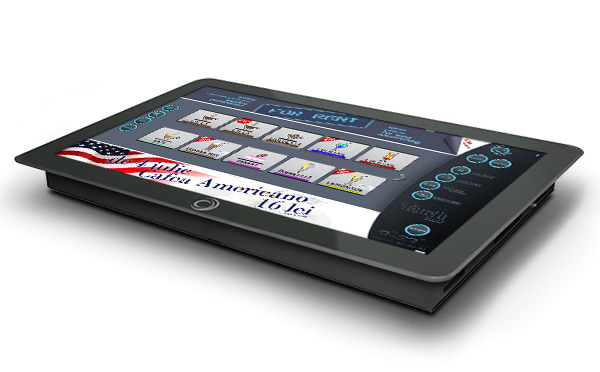
\includegraphics[width=\linewidth]{PCAP.png}
\caption{PCAP tables come with an interchangeable power cable and multi-language integration.}
\label{fig:PCAP}
\end{figure}

As far as usability goes, most users should be quick to learn how basic functions work, since multi-touch surfaces are nothing new for many users. The biggest obstacle for users may just be getting used to direct manipulation on such a large flat surface. However, I believe learnability, efficiency and memorability are three of its strongest metrics, as we are aiming for the most natural interface experience. Figure~\ref{fig:PCAP_restaurant} shows the PCAP table in an environment similar to a kitchen, and demonstrates how it can seamlessly blend into any tabletop.

\begin{figure}[ht]
\centering
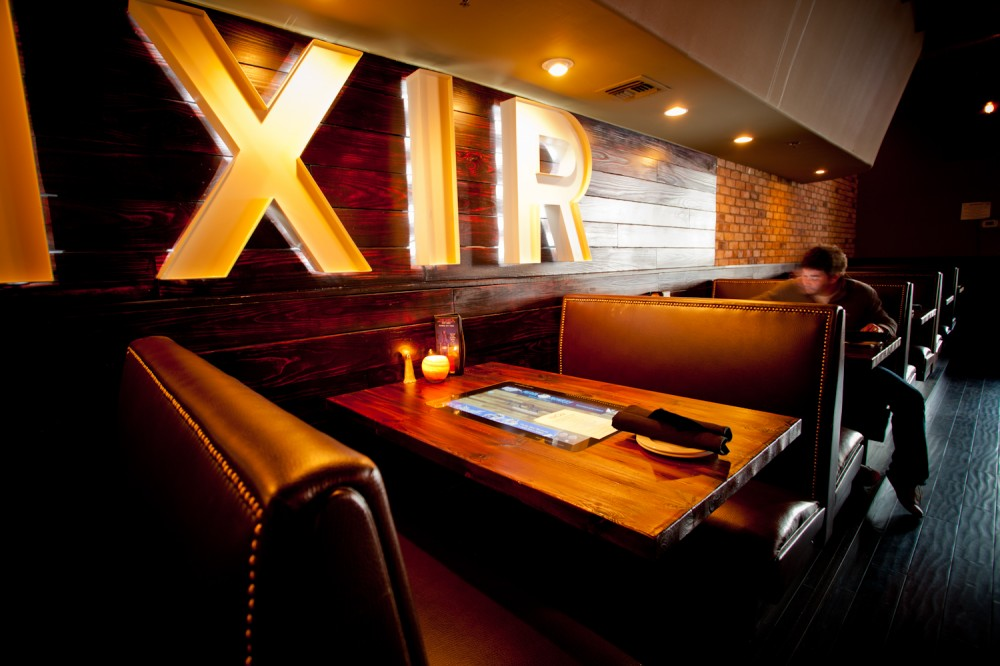
\includegraphics[width=\linewidth]{PCAP_restaurant.jpg}
\caption{The patented fixture system allows you to install this unit into any surface or wall with a few screws. Its edge to edge glass allows the PCAP to be placed into any type of table one could imagine.}
\label{fig:PCAP_restaurant}
\end{figure}

\section*{Top-level Design}
\subsection*{Basics}
When the Pomme Comptoir powers on, the user will see a blank screen with a default background image with an integrated date/time widget. For the sake of learnability and memorability, there will be a tool tip (with a disable option) that pops up on the screen telling the user how to begin. A user can open a new \emph{tile} by pressing and holding a single point on the screen. This will bring up a circular menu centered on the point. The menu will be evenly divided into three sections: YouTube, BigOven, and settings. To choose an option, the user may either drag his or her finger in the direction of the option or lift the finger and tap the option. As the user drags his or her finger towards an option, that particular chunk of the circle will \emph{fill up} with a bolder version of that chunk's color, giving the user an indication that he/she is choosing that option and that he/she has fully committed to choosing that option (if that is indeed the case).

\begin{figure}[ht]
\centering
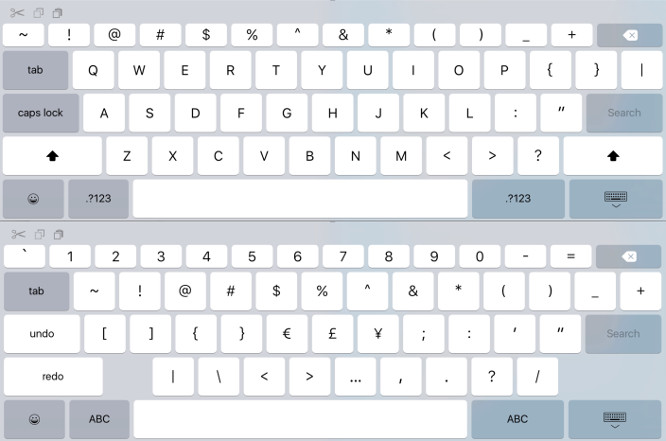
\includegraphics[width=\linewidth]{iOSkeyboard.jpg}
\caption{The on-screen keyboard will be similar in design and capability to the keyboards used for iOS devices.}
\label{fig:iOSkeyboard}
\end{figure}

\subsection*{Tiles}
Once the user chooses either YouTube or BigOven, a tile of a default size will open up and display a standard layout, which depends on the API being used. For both YouTube and BigOven, if a user has not logged in previously, both services will ask the user to login using either a Google or BigOven account.

It is important to note that there will be an implementation of an on-screen keyboard that is accessible to the user whenever text input is needed. This will be similar to an iOS keyboard, shown in Figure~\ref{fig:iOSkeyboard}. The keyboard will be in its own tile, thus it will be subject to all actions of a tile, which will be subsequently explained. However, there will be one important difference with the keyboard tile, in that it will have a string-like object attached to both it and the tile that is currently using the keyboard. This string will be slightly longer than the length between the two tiles, and will be subject to gravity and physics. This means that if the user were to drag either of the connected tiles, the other would be dragged along as well. Further, once another tile is selected by the user, the string would quickly detach from the previous tile and attach to the current one.

\subsubsection*{YouTube}
The standard YouTube layout will look and act like the mobile app, but with less of a focus on overall trending topics/videos. Instead, the design will promote and push videos that fall into the "cooking" category. Users will also have the ability to browse through his or her subscriptions or search for a video. The account information will also be accessible, which allows users to see his/her history, posted videos, and videos in playlists. The function offered by the YouTube API to upload videos will not be implemented. Selecting a video will open up a different layout that includes the video player, information about the video (title, description, view count, like/dislike buttons, account information), and related videos. The full screen function will use the entire tile instead of the entire screen, and any unused space in the tile will be black.

\subsubsection*{BigOven}
The BigOven layout will offer the four main services of the API, but will have its focus on the recipes and grocery lists, since images and reviews go hand in hand with recipes. There will be a search bar at the top of the tile, with tabs across the bottom for grocery lists, recipe lists, meal planner, and meal collections. The meal planner is a calendar that allows the user to plan out his/her meals by choosing which day will be reserved for each meal. The main screen will feature some trending recipes. Because the user is assumed to be logged into a BigOven account, his or her grocery list is expected to sync between devices. Thus, a user will be able to search for a recipe, view images related to that recipe, read/write reviews about that recipe, save it to his/her list of recipes, and add the ingredients to his/her grocery list. From there, a user could potentially go to the market, open up the BigOven mobile app and see the updated grocery list. Note: there will also be an option within the BigOven tile to simply have a timer or stopwatch service, which will take up the entire tile area. 

\subsubsection*{Settings}
The settings tile will be the hub for customization, giving users the option to change the main background, date and time zone/configuration, multi-touch gestures, screen brightness, volume, text size, accessibility settings, and parental controls. In addition, the tile will also display what accounts are logged into YouTube and BigOven at that time, giving the user the option to log out and/or log in.

\subsubsection*{Sizing, Closing, Clearing and Spreading Tiles}
Any tile may be re-sized by the user by pressing and dragging a corner or side of a tile. Additionally, a tile can be dragged by holding and dragging n$>$2 fingers that are in the window. The minimum size for any tile is 2" x 2". This is to say, at any point, neither dimension can be less than 2" long, e.g. 4" x 2" is acceptable, while 1" x 2" is not.

To close a tile, the default gesture will be a palm directly on the tile. If there are multiple tiles beneath the user's palm, the window that is above the others and/or is covered by the biggest percentage of the palm's area will be closed. Alternatively, a user can simply \emph{re-size} a tile out of existence by dragging a corner/side towards the opposite corner/side. The system will automatically re-size the tile to the minimum size unless the user drags the corner/side within 0.5" of the opposite corner/size.

If the screen gets cluttered with tiles, the user has an option to "clear out" the tiles by spreading with the thumb and 3+ fingers, which will fling all of them to the edges of the screen, allowing for the user to create a new tile by pressing and holding on the background. Furthermore, if the user wishes to see all currently open tiles, he/she can "spread out" the tiles by swiping up with 3+ fingers, causing them to decrease in size and spread out across the screen, making sure that every tile is fully visible. The user can then select one tile to bring to the front.

\section*{Usage Scenarios}
\subsection*{Learning a cooking technique from a video}
If a user wishes to improve his/her cooking skills, he/she may want to learn from watching a professional on YouTube. In this case, a user can open up a YouTube tile and search for a particular cooking technique, e.g. the correct way to cut vegetables. If a user would like to easily come back to this video, he/she can add it to a playlist, since he/she will already have been logged in.

\subsection*{Finding and preparing a recipe}
If a user plans to make dinner later on in the day, he/she can open up a BigOven tab, search for a recipe or select one from his/her saved recipes, then add the ingredients to his/her grocery list. Then he/she can visit the grocery store before dinner time and check the BigOven app on his/her mobile device and see the grocery list that was created earlier. Once the ingredients have been brought to the kitchen, the user can open up the recipe in a BigOven tile and resize it to see the entire set of instructions. If cooking in the oven or on the stove is required, he/she can use the built-in timer/stopwatch function included in the BigOven interface. Finally, after enjoying the meal, the user can write a review of the recipe in the same BigOven tile.

\section*{Rationale}
The goal behind Pomme Comptoir is to really expedite the cooking process. From discovering meals to learning how to cook, Pomme Comptoir is meant to get neophytes off the ground and make expert chefs more efficient. There seems to be a disconnect between bleeding-edge technology and food preparation, and Pomme Comptoir tries to fill that gap by giving instant access to recipes and tutorials right there in the kitchen.

The main priority for Pomme Comptoir would have to be increasing the efficiency of the user. With natural gestures we hope to give users a smooth experience, and the tile layout aims to give users that opportunity to multi-task, which is important in the busy kitchen environment. The mental model I hope to get across is one that is consistent with the style guides of many big developers, where I would want simplicity to reign while still allowing for a complex and diverse interaction. The use of tiles to symbolize the need for multi-tasking is a model that would hopefully be used competently. 

\section*{Usability Metric Forecast}
Starting with the weaker metrics, I believe Pomme Comptoir will be relatively weak in the error and learnability metrics, because of the fact that there will be no visual cues (other than the tool tips) to aid the user if it is their first time using the system. Furthermore, it may take some time to get used to the gestures and multi-touch system, which could make the potential for errors higher than usual.

However, I believe the memorability, efficiency and satisfaction metrics will be strong. This is because of the fact that users will most likely be using Pomme Comptoir on a weekly, if not daily, basis, which makes memorability strong. Efficiency is the name of the game for this interface, which is backed up by the implementation of natural multi-touch gestures and the tile system. Finally, I believe the satisfaction of the user will be high because of the streamlined cooking process Pomme Comptoir offers as well as the customization of the entire interface, from the background image to the size of tiles. 

\section*{Acknowledgments}

Dr. John David N. Dionisio

\begin{thebibliography}{5}

	%Each item starts with a \bibitem{reference} command and the details thereafter.
	\bibitem{DTS}
	Digital Touch Systems. "PCAP – Projected Capacitive Touch Tables." Digital Touch Systems. N.p., n.d. Web. $<$http://digitaltouchsystems.com/products/touch-screens-tables/pcap-touch-tables/$>$.

	\bibitem{YouTube}
	Google Developers. "YouTube Data API  |  Google Developers." Google Developers. N.p., n.d. Web. 25 Nov. 2015. $<$https://developers.google.com/youtube/v3/$>$.
    
    \bibitem{BigOven}
    BigOven. "BigOven API." 350,000+ Recipe and Grocery List API. N.p., n.d. Web. 25 Nov. 2015. $<$http://api.bigoven.com/$>$. 


\end{thebibliography}

\end{document}